\chapter{Zig-zag, DC prediction and run-length coding}\label{ch:zigzag}

After quantization each tile is 64 small integers, mostly zeros. This chapter turns them into a short list of ``events'' that the Huffman coder (next chapter) can write compactly.

\section{Zig-zag: sort by importance}

If we read the $8\times8$ tile row by row, the non-zero values are scattered among the zeros. If instead we read it along the anti-diagonals from the top-left corner outward, we visit coefficients roughly from \emph{lowest to highest frequency}. Since high frequencies are mostly zero, the zeros bunch up into one long run at the end.

\begin{figure}[h]
\centering
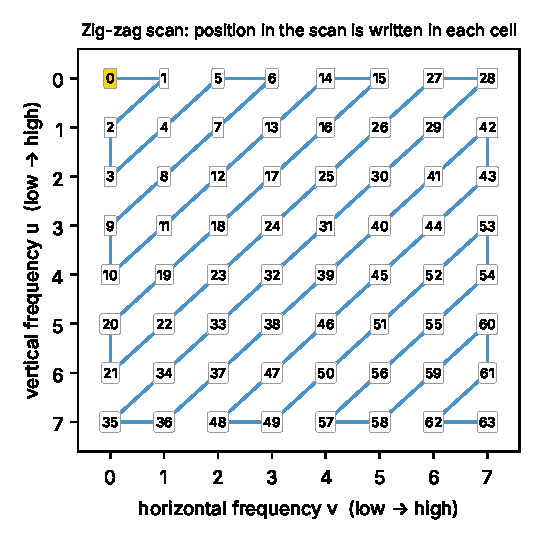
\includegraphics[width=0.46\textwidth]{figures/zigzag.pdf}
\caption{The zig-zag scan. Position 0 (gold) is the DC coefficient, 63 is the highest frequency. After quantization the tail of the scan is almost entirely zero.}
\end{figure}

The code builds the order by walking the 15 anti-diagonals ($\text{row}+\text{col}=s$), alternating direction:
\lstinputlisting{snippets/code_zigzag.cpp}
The test \code{zigzag\_is\_permutation\_and\_has\_jpeg\_prefix} checks that every index 0..63 appears exactly once and that the first sixteen entries equal the well-known JPEG sequence $0,1,8,16,9,2,3,10,17,24,\dots$

For our example tile the 64 numbers in zig-zag order are
\[
[34,\ 0,\ 6,\ -4,\ 0,\ 1,\ 0,\ -1,\ 0,\ 3,\ -2,\ 0,\ 0,\ 0,\ 0,\ 0,\ 0,\ 0,\ 0,\ 0,\ 1,\ 0,\ 0,\ 0,\ \dots]
\]
(the trailing zeros are all zero). Now it is obvious what the next step does: describe this list briefly.

\section{DC prediction: send differences}

Position 0 is the \emph{DC coefficient}, the tile's average brightness. Neighbouring tiles usually have similar averages (sky next to sky). So instead of the DC value we send its difference to the previous tile's DC. This is called \textbf{DPCM} (differential pulse-code modulation).

\begin{figure}[h]
\centering
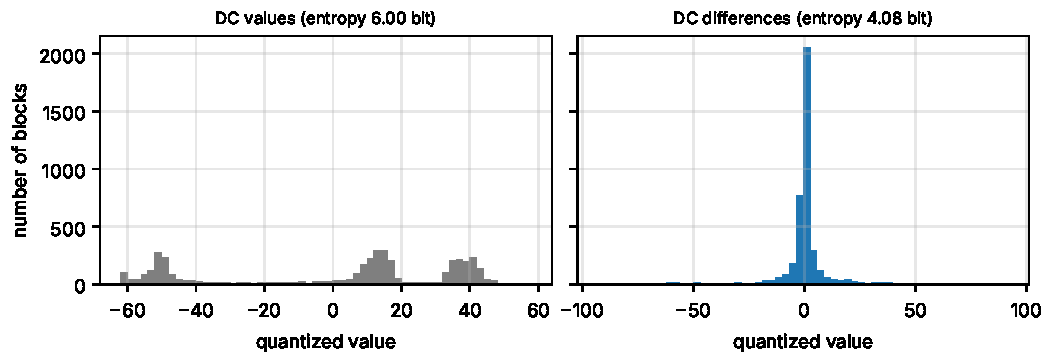
\includegraphics[width=0.85\textwidth]{figures/dc_prediction.pdf}
\caption{\label{fig:dc}Quantized DC values of the cameraman (left) are spread widely; their differences from the previous tile (right) cluster around zero. The entropy, a lower bound on bits per value for a simple code, drops from \dcEntropyRaw\ to \dcEntropyDiff\ bits.}
\end{figure}

\section{AC coefficients: (run, size) pairs}

For the 63 remaining values we do not list the zeros one by one. We list only the non-zero values and say how many zeros came before each. Each non-zero value is described by two things:

\begin{itemize}
\item \textbf{run}: the number of zeros since the last non-zero value (0--15),
\item \textbf{size} (``category''): the number of bits needed for its magnitude. Value 0 $\to$ category 0, $\pm1\to1$, $\pm2,\pm3\to2$, $\pm4..\pm7\to3$, and so on. (Code: \code{category()}.)
\end{itemize}

The pair $({\rm run},{\rm size})$ packs into one byte, $({\rm run}\ll4)\,|\,{\rm size}$, and \emph{that byte} is the symbol that gets a Huffman code. After the code come \code{size} raw bits that say exactly which value in the category it is.

\subsection{Amplitude bits: how negative numbers are stored}

In category 3 the possible magnitudes are 4..7, so the sign and magnitude together have 8 possibilities, and 3 bits suffice. JPEG's trick: positive values are written as themselves; a negative value $v$ is written as $v+(2^{\rm size}-1)$, i.e.\ the bitwise complement of its magnitude. For size~3: $4,5,6,7\to100,101,110,111$ and $-4,-5,-6,-7\to011,010,001,000$. The first bit of the amplitude therefore tells the sign (1 = positive). The decoder reverses this in \code{extendAmplitude}.

\subsection{Two special symbols}

\begin{description}
\item[EOB, end of block (\texttt{0x00}).] Sent as soon as all remaining coefficients are zero. This is the big win: a typical tile ends after a handful of values, and the whole zero tail costs one short code (3 bits in our example).
\item[ZRL, zero run length (\texttt{0xF0}).] The run field has only 4 bits (0..15). A stretch of 16 or more zeros is broken into one ZRL per 16 zeros, then a normal pair for the rest. If the last coefficient (position 63) is non-zero there are no trailing zeros and no EOB.
\end{description}

\lstinputlisting{snippets/code_rle.cpp}

\section{Our example tile, token by token}

Previous tile's DC was \exPrevDC. The tile in the example has quantized DC $34$, so we send the difference $34-\exPrevDC=-3$. The table shows every symbol sent for the tile, the actual Huffman codes the encoder used for the full cameraman at quality~50, and the bit cost:

\begin{center}
\small
\begin{tabular}{@{}llp{3.3cm}rllr@{}}
\toprule
 & symbol & meaning & value & Huffman code & amplitude & bits\\ \midrule
\inputrows{snippets/ex_tokens}
\end{tabular}
\end{center}

The whole tile costs \textbf{\exBlockBits\ bits} instead of $64\cdot8=512$ bits: a local ratio of about \exBlockRatio:1, on a tile with non-trivial detail.

\begin{plain}
\textbf{Check it yourself.} The value $6$ is in category 3, run 1 (one zero before it) $\Rightarrow$ symbol $(1\ll4)|3=\texttt{0x13}$, amplitude bits \texttt{110}. The value $-4$ is category 3, so it is stored as $-4+7=3=\texttt{011}$. After $-2$ there are 9 zeros, then a $1$ $\Rightarrow$ symbol $(9\ll4)|1=\texttt{0x91}$. Then nothing but zeros, so EOB.
\end{plain}

\begin{sound}
``After quantization a block is mostly zeros, so I read it in zig-zag order to group the zeros at the end, send the DC as a difference to the previous block, and code each non-zero AC value as a (run, size) symbol plus raw amplitude bits, with a special end-of-block symbol for the zero tail, exactly as baseline JPEG does.''
\end{sound}
